\documentclass[a4paper,12pt]{article}
\usepackage{amsmath,amssymb,amsfonts,amsthm}
\usepackage{tikz}
\usepackage[utf8x]{inputenc}
\usepackage[T2A]{fontenc} 
\usepackage[russian]{babel}
\usepackage{cmap} 
\usepackage{ gensymb }
% Так ссылки в PDF будут активны
\usepackage[unicode]{hyperref}
\usepackage{ textcomp }
\usepackage{indentfirst}
\usepackage[version=3]{mhchem}

% вы сможете вставлять картинки командой \includegraphics[width=0.7\textwidth]{ИМЯ ФАЙЛА}
% получается подключать, как минимум, файлы .pdf, .jpg, .png.
\usepackage{graphicx}
\usepackage{wrapfig}
% Если вы хотите явно указать поля:
\usepackage[margin=1in]{geometry}
% Или если вы хотите задать поля менее явно (чем больше DIV, тем больше места под текст):
% \usepackage[DIV=10]{typearea}

\usepackage{fancyhdr}

\newcommand{\bbR}{\mathbb R}%теперь вместо длинной команды \mathbb R (множество вещественных чисел) можно писать короткую запись \bbR. Вместо \bbR вы можете вписать любую строчку букв, которая начинается с '\'.
\newcommand{\eps}{\varepsilon}
\newcommand{\bbN}{\mathbb N}
\newcommand{\dif}{\mathrm{d}}

\newtheorem{Def}{Определение}


\pagestyle{fancy}
\makeatletter % сделать "@" "буквой", а не "спецсимволом" - можно использовать "служебные" команды, содержащие @ в названии
\fancyhead[L]{\footnotesize Лабораторные работы по общей физике}%Это будет написано вверху страницы слева
\fancyhead[R]{\footnotesize ФУПМ МФТИ}
%\fancyfoot[L]{\footnotesize \@author}%имя автора будет написано внизу страницы слева
\fancyfoot[R]{\thepage}%номер страницы —- внизу справа
\fancyfoot[C]{}%по центру внизу страницы пусто

\renewcommand{\maketitle}{%
	\noindent{\bfseries\scshape\large\@title\ \mdseries\upshape}\par
	\noindent {\large\itshape\@author}
	\vskip 2ex}
\makeatother
\def\dd#1#2{\frac{\partial#1}{\partial#2}}


\title{4.3. Измерение абсолютной активности препарата $^{60}Co$ методом $\gamma-\gamma$ совпадений.}
\author{Хурсик Екатерина} 
\date{\today}

\begin{document}
	
\maketitle
\section{Цель работы}

Определить абсолютную активность радиоактивного препарата $^{60}Co$ с использованием
каскадного перехода $\gamma$-квантов при его распаде.

\section{Метод достижения цели}

Чтобы определить абсолютную активность $^{60}Co$
\begin{itemize}
	\item измеряем полную скорость счёта и фон для каждого счётчика,
	\item вычисляем истинные скорости счёта каждого источника как разность полной скорости счёта и фона,
	\item в режиме совпадений измеряем полное число совпадений и число случайных совпадений,
	\item вычисляем скорость истинных совпадений $N_\text{совп}$ как их разность,
	\item по формуле (1) находим абсолютную активность кобальта.
\end{itemize}

\section{Ход работы}

\subsection{}

Вначале проведём проверку работоспособности установки. Будем подносить один из блоков
ФЭУ к источнику $^{60}Co$, затем уберём его. Наблюдаем изменение скорости счёта по
пересчётному прибору (т.е. установка "чувствует" присутствие $\gamma$-источника).
Повторяем те же действия со вторым блоком ФЭУ.

\subsection{}

Отодвинем ФЭУ подальше от источника и измерим фон этого счётчика с точностью 
порядка 1\%. Те же измерения проведём со вторым счётчиком.
\begin{equation*}
	n_{1_\text{ф}}=18,72,\quad\quad n_{2_\text{ф}}=61,68.
\end{equation*}

\subsection{}

Установим источник $^{60}Co$ между двумя счётчиками и измерим полную скорость счёта
в первом и во втором счётчиках с точностью порядка 0,5\%.
\begin{equation*}
	n_{1_\text{п}}=2661,07,\quad\quad n_{2_\text{п}}=2341,2.
\end{equation*}
Затем по имеющимся полной скорости счёта и фону рассчитаем для каждого счётчика
по формулам
\begin{equation*}
	N_1=n_{1_\text{п}}-n_{1_\text{ф}}\quad\quad N_2=n_{2_\text{п}}-n_{2_\text{ф}}
\end{equation*}
Все результаты измерений занесём в таблицу
$$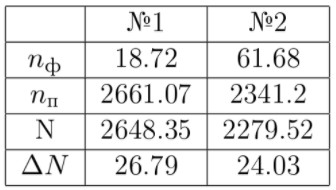
\includegraphics[width=0.35\linewidth]{2020-12-03-1.jpg}$$

\subsection{}

Включим прибор СС в режим совпадений и измерим скорости счёта совпадений для всех
разрешающих времён, указанных на приборе, с точностью порядка 1\%.
Определим $N_0$ в Ки по формуле
\begin{equation}
	N_0=1,08\frac{N_1N_2}{2N_\text{совп}}
\end{equation}
для всех щначений разрешающих времён $\tau$.\\
Результаты измерений занесём в таблицу.
$$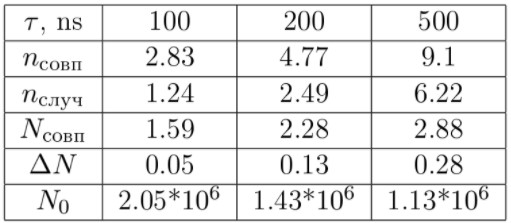
\includegraphics[width=0.5\linewidth]{2020-12-03-2.jpg}$$
Построим график зависимости $N_0$ и $\tau$.
$$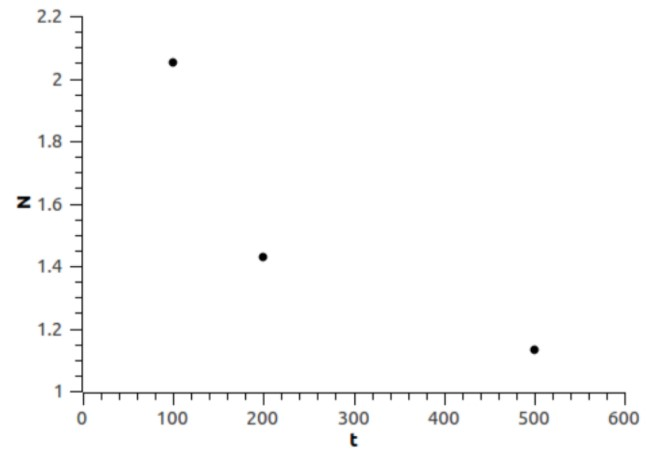
\includegraphics[width=0.7\linewidth]{2020-12-03-3.jpg}$$

\end{document}
